\documentclass[border=6pt]{standalone}
\usepackage{amsmath}
\usepackage{amssymb}
\usepackage{tikz}
\usepackage{pgfplots}
\pgfplotsset{compat=1.18}
\usetikzlibrary{arrows.meta,calc,positioning}
\begin{document}
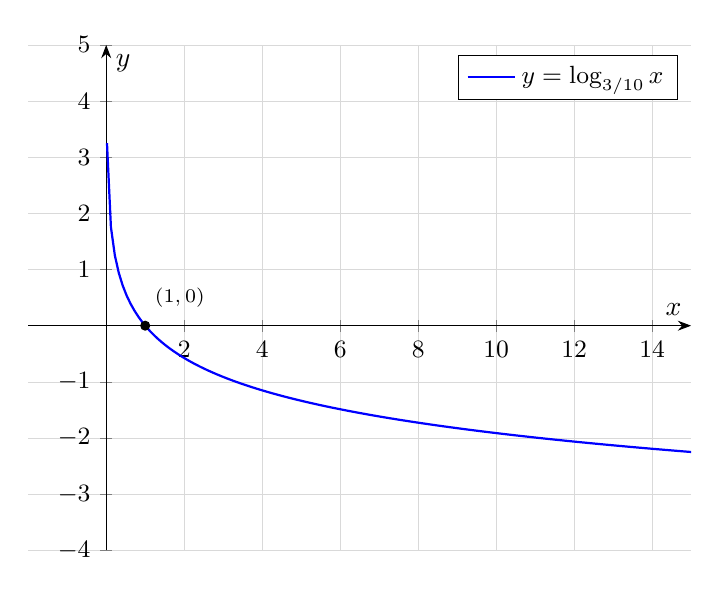
\begin{tikzpicture}
\begin{axis}[
    axis lines = middle,
    xlabel = {$x$}, ylabel = {$y$},
    grid=both,
    grid style={line width=.1pt, draw=gray!30},
    axis line style={-Stealth},
    legend style={font=\small},
    tick label style={font=\small},
    xmin=-2, xmax=15, ymin=-4, ymax=5,
    xtick={0,2,4,6,8,10,12,14},
    ytick={-4,-3,-2,-1,0,1,2,3,4,5},
    width=10cm, height=8cm,
]
\addplot[domain=0.02:15, samples=150, thick, blue] {ln(x)/ln(0.3)};
\addlegendentry{$y=\log_{3/10} x$}
\addplot[only marks, mark=*, mark size=1.6pt, black] coordinates {(1,0)};
\node[anchor=south west, font=\scriptsize] at (axis cs:1,0.15) {$(1,0)$};
\end{axis}
\end{tikzpicture}
\end{document}
